\documentclass[11pt,a4paper]{article}
\usepackage[margin=1in]{geometry}
\usepackage[T1]{fontenc}
\usepackage[utf8]{inputenc}
\usepackage{lmodern}
\usepackage{hyperref}
\usepackage{enumitem}
\usepackage{xurl}
\usepackage{tikz}
\usepackage{float}
\usetikzlibrary{arrows.meta, positioning, shapes.geometric}
\hypersetup{colorlinks=true,linkcolor=blue,urlcolor=blue}
\newcommand{\codepath}[1]{\path{#1}}
\tikzset{box/.style={rectangle,draw,rounded corners,align=center,inner sep=3pt,minimum width=36mm},line/.style={-Latex}}

\title{Phase-1 Deliverable: Trace Ingestion API}
\author{SIT Engine Architecture}
\date{\today}

\begin{document}
\maketitle

\section{Technical Description}
Trace Ingestion API is the anti-coupling contract that separates source parsing from engine logic. It defines normalized state/residency schemas and adapter interfaces.

\section{Implementation Fulfillment}
Contract and validators are implemented in \codepath{Phase-1/ingest/ingest_api.py} (\texttt{TraceAdapter}, \texttt{validate\_state\_df}, \texttt{validate\_resid\_df}). Engine usage is through \codepath{Phase-1/adapters/baseline_adapter.py} in \codepath{Phase-1/sit_engine_phase1.py}.

\section{Design \& Architecture}
Adapters parse source-specific traces and emit normalized DataFrames. The engine consumes only normalized events; adding new targets requires new adapters, not engine changes.

\subsection*{Function Flowchart}
\begin{figure}[H]
\centering
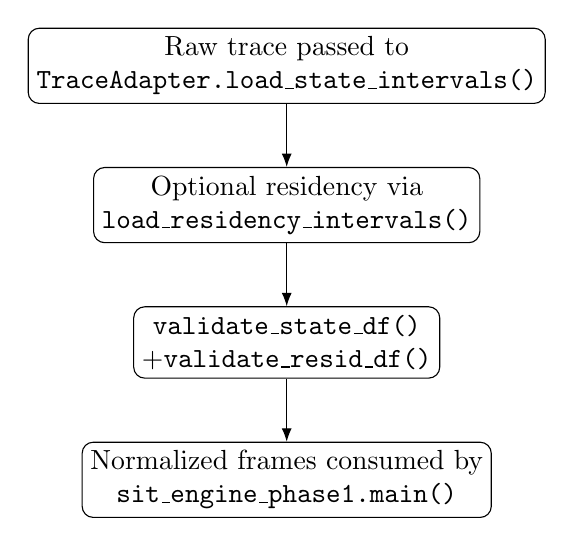
\begin{tikzpicture}[node distance=8mm and 12mm]
\node[box] (a) {Raw trace passed to\\\texttt{TraceAdapter.load\_state\_intervals()}};
\node[box, below=of a] (b) {Optional residency via\\\texttt{load\_residency\_intervals()}};
\node[box, below=of b] (c) {\texttt{validate\_state\_df()}\\+\texttt{validate\_resid\_df()}};
\node[box, below=of c] (d) {Normalized frames consumed by\\\texttt{sit\_engine\_phase1.main()}};
\draw[line] (a) -- (b);
\draw[line] (b) -- (c);
\draw[line] (c) -- (d);
\end{tikzpicture}
\caption{Trace Ingestion API Function Flow}
\end{figure}

\end{document}
